\chapter{Evaluation}
\label{chp:eval}

\section{Experimental Setup}

%, using the Docker-based environment described in Chapter~\ref{chp:docker}.

The evaluation of the tool was carried out on a local machine.  
The experimental environment consisted of:

\begin{myitemize}
    \item Local machine running \textbf{Ubuntu 25.04};
    %\item Docker container based on \textbf{Ubuntu 24.04};
    \item \textbf{Ghidra~11.4.2} (latest version at the time of evaluation);
    \item \textbf{Jadx~1.5.3} (latest version at the time of evaluation);
    \item \textbf{GhidraMCP~1.4} (latest version at the time of evaluation);
    \item \textbf{jadx-ai-mcp~4.0.0} (latest version at the time of evaluation).
\end{myitemize}

\subsection{AWS for POIROT}

The extraction of crashes used for this evaluation is described in Chapter~\ref{chp:preliminaries}, and the corresponding execution environment is detailed in Chapter~\ref{chp:preliminaries_env}.  
All POIROT runs were executed on an AWS EC2 instance configured for large-scale fuzzing.

\subsection{\glsxtrshort{llm} Used}

The evaluation was conducted using the OpenAI model GPT-5.1.  
This model represented one of the most capable \glspl{llm} available at the time of testing and offered reliable support for \gls{mcp}-based tool use.
GPT-5.1 also integrates smoothly with the Pydantic framework, allowing strict control over structured outputs.

% No fine-tuning or additional training was performed, as the goal of the evaluation was to assess how a general-purpose model behaves when equipped with structured context and targeted guidance through MCP-based evidence retrieval.


\section{Test Applications}

Table~\ref{tab:apps} lists the applications used for the evaluation, together with the exact versions of each APK.  
These apps were selected from the POIROT dataset and filtered based on the run performed. %The applications may have different versions in the POIROT dataset and this dataset. \textcolor{red}{Non so se tenere questa ultima frase per sengalare che le apks hanno versioni diverse}

\begin{table}[ht]
\centering
\resizebox{1\textwidth}{!}{
\begin{tabular}{|l|l||l|l|}
\hline
%\multicolumn{4}{|c|}{\textbf{Applications Used for Evaluation}} \\
%\hline
\textbf{App} & \textbf{Version} & \textbf{App} & \textbf{Version} \\
\hline
br.com.pedidos10 & 1.16.4 & ca.radioplayer.android & 6.3.420.1 \\
com.ahnlab.v3mobileplus & 2.5.20.10 & com.appgeneration.itunerfree & 9.3.13 \\
com.cisco.webex.meetings & 45.3.0 & com.clearchannel.iheartradio.controller & 10.36.0 \\
com.ford.fordpasseu & 4.23.1 & com.hyundaicard.cultureapp & 1.0.72 \\
com.intsig.BCRLite & 7.85.5 & com.jeju.genie & 2.2.13 \\
com.kbstar.kbbridge & 1.2.1 & com.kt.ktauth & 02.01.37 \\
com.lottemembers.android & 7.7.5 & com.more.dayzsurvival.gp & 25.1002.1 \\
com.pandora.android & 2509.1 & com.rockbite.deeptown & 6.2.10 \\
com.rstgames.durak & 1.9.11 & com.samsungcard.shopping & 1.4.901 \\
com.skmc.okcashbag.home\_google & 7.0.8 & com.skt.prod.dialer & 13.6.5 \\
com.skt.smartbill & 6.4.1 & com.sopheos.videgreniersmobile & 20.11.10 \\
com.ssg.serviceapp.android.egiftcertificate & 2.6.10 & com.teamjin.deliveryk & 7.0.3 \\
com.tencent.mm & 8.0.28 & com.tplink.skylight & 3.1.20 \\
fr.radioplayer.android & 6.6.420.1 & kr.co.busanbank.mbp & 3.0.10 \\
kr.co.morpheus.geps & 02.42 & kr.co.samsungcard.mpocket & 5.4.306 \\
kr.go.iros & 1.2.3 & kr.go.kcs.mobile.pubservice & 1.0.281 \\
kr.go.minwon.m & 2.5.95 & kr.go.nts.android & 12.8 \\
kr.go.wetax.android & 5.4.14 & nh.smart.allonebank & 1.8.8 \\
nh.smart.banking & 4.1.2 & nh.smart.card & 6.5.0 \\
nh.smart.nhcok & 2.0.70 & ragazzo.alphacode.com.br & 3.0.9 \\
tw.com.taishinbank.ccapp & 5.631 & tw.gov.tra.twtraffic & 2.1.2 \\
\hline
\end{tabular}
}
\caption{Applications evaluated by the triage system.}
\label{tab:apps}
\end{table}

Across all these applications, a total of 59 methods were identified, each associated with one or more crashes.  
%In total, the dataset contained 134 crash instances.

\subsection{Execution Time}

Table~\ref{tab:apps_time} reports the \gls{llm}-analysis time for each application.  
The total time per APK depends primarily on the \emph{number of crashes} produced by POIROT, as well as the number of relevant libraries and the complexity of the stack trace.
Note that the reported time covers only the \gls{llm} classification phase and does not include the startup time of Ghidra, which depends solely on the number and size of the native libraries being imported.

\begin{table}[ht]
\centering
\resizebox{1\textwidth}{!}{
\begin{tabular}{|l|l||l|l|}
\hline
%\multicolumn{4}{|c|}{\textbf{Execution LLM Time per Application}} \\
%\hline
\textbf{App} & \textbf{Time (s)} & \textbf{App} & \textbf{Time (s)} \\
\hline
br.com.pedidos10 & 80 & ca.radioplayer.android & 480 \\ 
com.ahnlab.v3mobileplus & 338 & com.appgeneration.itunerfree & 113 \\ 
com.cisco.webex.meetings & 129 & com.clearchannel.iheartradio.controller & 200 \\ 
com.ford.fordpasseu & 185 & com.hyundaicard.cultureapp & 48 \\ 
com.intsig.BCRLite & 59 & com.jeju.genie & 33 \\ 
com.kbstar.kbbridge & 35 & com.kt.ktauth & 28 \\ 
com.lottemembers.android & 71 & com.more.dayzsurvival.gp & 25 \\ 
com.pandora.android & 420 & com.rockbite.deeptown & 17 \\ 
com.rstgames.durak & 36 & com.samsungcard.shopping & 22 \\ 
com.skmc.okcashbag.home\_google & 57 & com.skt.prod.dialer & 278 \\ 
com.skt.smartbill & 579 & com.sopheos.videgreniersmobile & 60 \\ 
com.ssg.serviceapp.android.egiftcertificate & 31 & com.teamjin.deliveryk & 83 \\ 
com.tencent.mm & 321 & com.tplink.skylight & 71 \\ 
fr.radioplayer.android & 628 & kr.co.busanbank.mbp & 805 \\ 
kr.co.morpheus.geps & 59 & kr.co.samsungcard.mpocket & 55 \\ 
kr.go.iros & 43 & kr.go.kcs.mobile.pubservice & 60 \\ 
kr.go.minwon.m & 30 & kr.go.nts.android & 87 \\ 
kr.go.wetax.android & 35 & nh.smart.allonebank & 36 \\ 
nh.smart.banking & 29 & nh.smart.card & 30 \\ 
nh.smart.nhcok & 37 & ragazzo.alphacode.com.br & 87 \\ 
tw.com.taishinbank.ccapp & 98 & tw.gov.tra.twtraffic & 78 \\ 

\hline
\hline
\multicolumn{2}{|r||}{\textbf{Average Time}} & \multicolumn{2}{l|}{\textbf{142}} \\
\hline
\end{tabular}
}
\caption{LLM analysis time per application.}
\label{tab:apps_time}
\end{table}

\subsection{Tokens usage}

\glspl{llm}, when accessed through their cloud \glspl{api}, compute usage costs based on the number of \emph{input tokens} (the prompt sent to the model) and \emph{output tokens} (the generated response).  
Token consumption plays a central role in both performance and cost.  
In this evaluation, usage varies primarily according to the size of the prompts (which include both the system and user components), the number of crashes produced by POIROT for each application, the amount of decompiled code retrieved from Ghidra—which grows with the depth and complexity of the stack trace—and the verbosity of the final triage explanation generated by the \gls{llm}.  


Table~\ref{tab:apps_tokens} reports input and output token usage for each application.

\begin{table}[ht]
\centering
\resizebox{1\textwidth}{!}{
\begin{tabular}{|l|l|l||l|l|l|}
\hline
%\multicolumn{6}{|c|}{\textbf{Token Usage per Application}} \\
%\hline
\textbf{App} & \textbf{Input} & \textbf{Output} &
\textbf{App} & \textbf{Input} & \textbf{Output} \\
\hline
br.com.pedidos10 & 36344 & 4006 & ca.radioplayer.android & 494465 & 23484 \\ 
com.ahnlab.v3mobileplus & 392719 & 17831 & com.appgeneration.itunerfree & 53776 & 6516 \\ 
com.cisco.webex.meetings & 92548 & 7643 & com.clearchannel.iheartradio.controller & 151439 & 7039 \\ 
com.ford.fordpasseu & 84360 & 6811 & com.hyundaicard.cultureapp & 14153 & 2152 \\ 
com.intsig.BCRLite & 33230 & 4095 & com.jeju.genie & 12987 & 2244 \\ 
com.kbstar.kbbridge & 13014 & 2189 & com.kt.ktauth & 41470 & 1466 \\ 
com.lottemembers.android & 38747 & 2655 & com.more.dayzsurvival.gp & 6542 & 1250 \\ 
com.pandora.android & 70891 & 9638 & com.rockbite.deeptown & 6564 & 1421 \\ 
com.rstgames.durak & 19232 & 1726 & com.samsungcard.shopping & 12380 & 1170 \\ 
com.skmc.okcashbag.home\_google & 30012 & 3708 & com.skt.prod.dialer & 212223 & 12100 \\ 
com.skt.smartbill & 359973 & 28820 & com.sopheos.videgreniersmobile & 48392 & 3213 \\ 
com.ssg.serviceapp.android.egiftcertificate & 18401 & 1734 & com.teamjin.deliveryk & 31816 & 4143 \\ 
com.tencent.mm & 877501 & 16197 & com.tplink.skylight & 29527 & 4077 \\ 
fr.radioplayer.android & 202292 & 21668 & kr.co.busanbank.mbp & 495055 & 44584 \\ 
kr.co.morpheus.geps & 22248 & 1544 & kr.co.samsungcard.mpocket & 29228 & 2915 \\ 
kr.go.iros & 24988 & 2374 & kr.go.kcs.mobile.pubservice & 25362 & 3232 \\ 
kr.go.minwon.m & 14516 & 1378 & kr.go.nts.android & 59025 & 4887 \\ 
kr.go.wetax.android & 12829 & 2305 & nh.smart.allonebank & 24960 & 1695 \\ 
nh.smart.banking & 20250 & 1610 & nh.smart.card & 14111 & 1783 \\ 
nh.smart.nhcok & 14361 & 1676 & ragazzo.alphacode.com.br & 38671 & 3792 \\ 
tw.com.taishinbank.ccapp & 31781 & 4205 & tw.gov.tra.twtraffic & 42834 & 3530 \\ 

\hline
\hline
\multicolumn{3}{|r||}{\textbf{Average Input Tokens}} &
\multicolumn{3}{l|}{\textbf{212434}} \\
\multicolumn{3}{|r||}{\textbf{Average Output Tokens}} &
\multicolumn{3}{l|}{\textbf{13963}} \\
\hline
\end{tabular}
}
\caption{Input and output token usage per application.}
\label{tab:apps_tokens}
\end{table}

\subsection{Requests and Tool Calls}

Each crash triggers a series of \emph{LLM requests}, corresponding to the number of times the agent sends a prompt to the model, and a number of \emph{LLM tool calls}, which represent successful invocations of Jadx or Ghidra through MCP during the analysis.  

Table~\ref{tab:apps_requests} reports, for each application, the number of LLM requests and MCP tool calls performed during the full triage stage.  

\begin{table}[ht]
\centering
\resizebox{1\textwidth}{!}{
\begin{tabular}{|l|l|l||l|l|l|}
\hline
%\multicolumn{6}{|c|}{\textbf{LLM request and Tool Calls per Application}} \\
%\hline
\textbf{App} & \textbf{Input} & \textbf{Output} &
\textbf{App} & \textbf{Input} & \textbf{Output} \\
\hline
br.com.pedidos10 & 5 & 9 & ca.radioplayer.android & 44 & 53 \\ 
com.ahnlab.v3mobileplus & 31 & 42 & com.appgeneration.itunerfree & 6 & 14 \\ 
com.cisco.webex.meetings & 10 & 23 & com.clearchannel.iheartradio.controller & 17 & 20 \\ 
com.ford.fordpasseu & 9 & 26 & com.hyundaicard.cultureapp & 2 & 3 \\ 
com.intsig.BCRLite & 4 & 9 & com.jeju.genie & 2 & 3 \\ 
com.kbstar.kbbridge & 2 & 3 & com.kt.ktauth & 6 & 6 \\ 
com.lottemembers.android & 2 & 5 & com.more.dayzsurvival.gp & 2 & 3 \\ 
com.pandora.android & 8 & 20 & com.rockbite.deeptown & 2 & 2 \\ 
com.rstgames.durak & 3 & 3 & com.samsungcard.shopping & 2 & 2 \\ 
com.skmc.okcashbag.home\_google & 4 & 5 & com.skt.prod.dialer & 26 & 26 \\ 
com.skt.smartbill & 51 & 82 & com.sopheos.videgreniersmobile & 6 & 10 \\ 
com.ssg.serviceapp.android.egiftcertificate & 3 & 2 & com.teamjin.deliveryk & 4 & 9 \\ 
com.tencent.mm & 49 & 42 & com.tplink.skylight & 4 & 9 \\ 
fr.radioplayer.android & 22 & 59 & kr.co.busanbank.mbp & 55 & 63 \\ 
kr.co.morpheus.geps & 3 & 4 & kr.co.samsungcard.mpocket & 4 & 8 \\ 
kr.go.iros & 4 & 4 & kr.go.kcs.mobile.pubservice & 4 & 4 \\ 
kr.go.minwon.m & 2 & 4 & kr.go.nts.android & 8 & 13 \\ 
kr.go.wetax.android & 2 & 3 & nh.smart.allonebank & 4 & 4 \\ 
nh.smart.banking & 3 & 4 & nh.smart.card & 2 & 3 \\ 
nh.smart.nhcok & 2 & 4 & ragazzo.alphacode.com.br & 5 & 13 \\ 
tw.com.taishinbank.ccapp & 4 & 10 & tw.gov.tra.twtraffic & 5 & 13 \\ 

\hline
\hline
\multicolumn{3}{|r||}{\textbf{Average LLM requests}} &
\multicolumn{3}{l|}{\textbf{16.4}} \\
\multicolumn{3}{|r||}{\textbf{Average LLM Tool Calls}} &
\multicolumn{3}{l|}{\textbf{25.3}} \\
\hline
\end{tabular}
}
\caption{LLM request and Tool Calls per application.}
\label{tab:apps_requests}
\end{table}
        
\vfill


\section{Evaluation Metrics}
%\textcolor{red}{non se serve specificare le metriche}


To objectively assess the performance of the \gls{llm}-based triage system, standard information retrieval metrics derived from a confusion matrix are employed. Given the binary nature of the classification task, determining whether a crash is a vulnerability or not, the possible outcomes are defined as follows:

\begin{itemize}
    \item \textbf{True Positive (TP):} A vulnerability correctly identified by the model. The crash represents a security risk, and the system correctly classified it as such (\texttt{is\_vulnerable: true}).
    \item \textbf{False Positive (FP):} A benign crash incorrectly flagged as a vulnerability. This represents a ''false alarm``, where the model assigns security relevance to a non-exploitable issue.
    \item \textbf{True Negative (TN):} A benign crash correctly identified as non-vulnerable. The system correctly determined that the issue does not pose a security risk.
    \item \textbf{False Negative (FN):} A vulnerability missed by the model. The crash is dangerous, but the system incorrectly classified it as benign.
\end{itemize}

Based on these definitions, the following metrics were calculated:

\paragraph{Accuracy}
Accuracy quantifies how many of the analysed crashes were assigned the correct label.  
It provides an overall view of the system’s correctness across both vulnerable and non-vulnerable cases.

\[
\text{Accuracy} = \frac{\text{TP} + \text{TN}}{\text{TP} + \text{TN} + \text{FP} + \text{FN}}
\]

\paragraph{Precision} Precision quantifies the reliability of the positive predictions. In the context of this thesis, high precision implies that when the tool flags a crash as a vulnerability, it is highly likely to be a real threat.
\[
\text{Precision} = \frac{\text{TP}}{\text{TP} + \text{FP}}
\]

\paragraph{Recall}
Recall measures how effectively the system identifies all crashes that correspond to real vulnerabilities.  
It captures the proportion of dangerous flaws that the model successfully flags.  

\[
\text{Recall} = \frac{\text{TP}}{\text{TP} + \text{FN}}
\]

\paragraph{F1-Score}
For the evaluation, the F1-score was selected as the primary metric. This measure is commonly employed in classification settings because it offers a single value that reflects the trade-off between precision and recall, which is especially important when the distribution of classes is unbalanced or when both false positives and false negatives carry comparable weight. The F1-score is defined as the harmonic mean of precision and recall:
\[
\mathrm{F1} = 2 \cdot \frac{\text{precision} \cdot \text{recall}}{\text{precision} + \text{recall}}
\]
The F1-score ensures a lower overall score if either precision or recall diverges significantly, even if one of the two is high, providing a balanced view of the model's effectiveness.

\section{Results}

\begin{comment}
    \begin{figure}[ht]
\centering
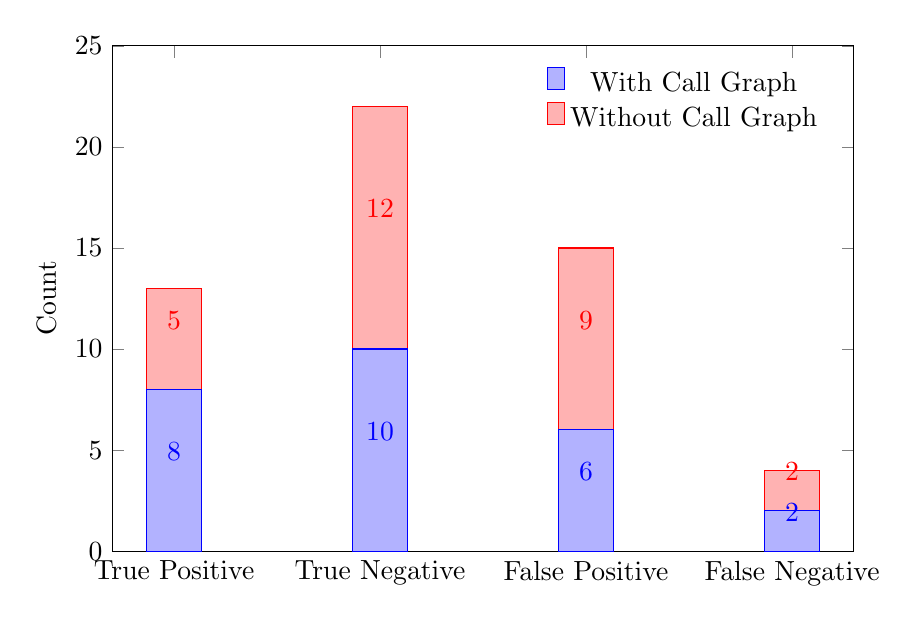
\begin{tikzpicture}
\begin{axis}[
    ybar stacked,
    ymin=0,
    ymax=25,
    bar width=20pt,
    width=11cm,
    height=8cm,
    ylabel={Count},
    symbolic x coords={TP,TN,FP,FN},
    xticklabels={
        {True~Positive},
        {True~Negative},
        {False~Positive},
        {False~Negative}
    },
    xtick=data,
    nodes near coords,
    nodes near coords align={vertical},
    legend style={
        at={(0.97,0.97)},
        anchor=north east,
        draw=none,
        fill=none
    },
    legend entries={{With Call Graph},{Without Call Graph}}
    %title={Triage Classification Outcomes},
]
\addplot coordinates {(TP,8) (TN,10) (FP,6) (FN,2)};
\addplot coordinates {(TP,5) (TN,12) (FP,9) (FN,2)};
\end{axis}
\end{tikzpicture}


\label{fig:classification_outcomes}
\end{figure}
\end{comment}

\begin{figure}
    \centering
    \begin{subfigure}{0.32\textwidth}
\scalebox{0.75}{
\begin{tabular}{c >{\bfseries}r @{\hspace{0.7em}}c 
                @{\hspace{0.4em}}c @{\hspace{0.7em}}l}
  \multirow{10}{*}{\rotatebox{90}{
      \parbox{6.2cm}{\bfseries\centering Actual\\}}} &
      & \multicolumn{2}{c}{\hspace*{-1em}\bfseries Predict} & \\
  & & \bfseries P & \bfseries N \\
  & P$'$ & \MyGradeColor{13}{21} & \MyGradeColor{3}{5} \\[2.1em]
  & N$'$ & \MyGradeColor{11}{18} & \MyGradeColor{34}{56} \\
% & P$'$ & \MyGradeColor{True}{Positive}{1} & \MyGradeColor{False}{Negative}{1} \\[2.1em]
% & N$'$ & \MyGradeColor{False}{Positive}{1} & \MyGradeColor{True}{Negative}{99} \\
\end{tabular}
}
\subcaption{Evaluation on methods that include a JCG}
\end{subfigure}
\hfill
\begin{subfigure}{0.32\textwidth}
\scalebox{0.75}{
\begin{tabular}{c >{\bfseries}r @{\hspace{0.7em}}c 
                @{\hspace{0.4em}}c @{\hspace{0.7em}}l}
  \multirow{10}{*}{\rotatebox{90}{
      \parbox{6.2cm}{\bfseries\centering Actual\\}}} &
      & \multicolumn{2}{c}{\hspace*{-1em}\bfseries Predict} & \\
  & & \bfseries P & \bfseries N \\
  & P$'$ & \MyGradeColor{10}{13} & \MyGradeColor{2}{3} \\[2.1em]
  & N$'$ & \MyGradeColor{30}{40} & \MyGradeColor{33}{44} \\
% & P$'$ & \MyGradeColor{True}{Positive}{1} & \MyGradeColor{False}{Negative}{1} \\[2.1em]
% & N$'$ & \MyGradeColor{False}{Positive}{1} & \MyGradeColor{True}{Negative}{99} \\
\end{tabular}
}
\subcaption{Evaluation on methods that do not include a JCG}
\end{subfigure}
\hfill
\begin{subfigure}{0.32\textwidth}
\scalebox{0.75}{
\begin{tabular}{c >{\bfseries}r @{\hspace{0.7em}}c 
                @{\hspace{0.4em}}c @{\hspace{0.7em}}l}
  \multirow{10}{*}{\rotatebox{90}{
      \parbox{6.2cm}{\bfseries\centering Actual\\}}} &
      & \multicolumn{2}{c}{\hspace*{-1em}\bfseries Predict} & \\
  & & \bfseries P & \bfseries N \\
  & P$'$ & \MyGradeColor{23}{17} & \MyGradeColor{5}{4} \\[2.1em]
  & N$'$ & \MyGradeColor{41}{30} & \MyGradeColor{67}{49} \\
% & P$'$ & \MyGradeColor{True}{Positive}{1} & \MyGradeColor{False}{Negative}{1} \\[2.1em]
% & N$'$ & \MyGradeColor{False}{Positive}{1} & \MyGradeColor{True}{Negative}{99} \\
\end{tabular}
}
\subcaption{Overall evaluation across the full set of methods}
\end{subfigure}
    \caption[Performance metrics for the vulnerability classification task]%
{Performance metrics for the vulnerability classification task.}
    \label{fig:classification_outcomes}
\end{figure}


The confusion matrices in Figure~\ref{fig:classification_outcomes} summarise how the system classified the 59 methods in the dataset, separating the two experimental conditions (with and without the \glsxtrlong{jcg}) and also reporting the aggregated results.

When the call graph is available, the system correctly identifies 8 vulnerabilities (TP) and misses 2 (FN), while producing 7 false alarms (FP) and 12 correct rejections (TN).  
Without the call graph, the model still detects 5 vulnerabilities and misses 2, but generates a higher number of false positives (9), with 12 true negatives.

Considering the dataset as a whole, the system reports 13 true positives and 24 true negatives, against 16 false positives and 4 false negatives.  
This distribution shows a clear tendency towards recall: the model successfully captures most real vulnerabilities, but at the cost of an increased number of false alarms, particularly when Java-side context is absent.


\begin{table}[ht]
\centering
\begin{tabular}{|p{2cm}|p{2.5cm}|p{2.5cm}|p{2.5cm}|}
\hline 
\centering \textbf{Metric} 
& \centering \textbf{With \glsxtrshort{jcg}} 
& \centering \textbf{Without \glsxtrshort{jcg}} 
& \centering \textbf{All APKs} \tabularnewline
\hline
\hline

\centering \textbf{Accuracy}  
& \centering 69.23~\% 
& \centering 60.71~\% 
& \centering 64.91~\% \tabularnewline

\centering \textbf{Recall}    
& \centering 57.14~\% 
& \centering 35.71~\% 
& \centering 44.83~\% \tabularnewline

\centering \textbf{Precision} 
& \centering 80.00~\% 
& \centering 71.43~\% 
& \centering 76.47~\% \tabularnewline

\centering \textbf{F1-Score}  
& \centering 66.67~\% 
& \centering 47.62~\% 
& \centering 56.52~\% \tabularnewline
\hline
\end{tabular}

\caption{Evaluation metrics computed from the classification results.}
\label{tab:eval_metrics}
\end{table}


Figure~\ref{fig:classification_outcomes} summarises the overall performance of the system. 
The aggregated accuracy (66.18~\%) indicates that roughly two-thirds of all crash classifications match the ground truth. 
A closer look at the two configurations reveals that accuracy is slightly higher when the call graph is available (68.75~\%) than when it is not (65.38~\%), suggesting that access to Java–to–native context provides a modest but tangible benefit.

Recall shows a more pronounced difference.  
With the call graph, the system successfully recovers 80.00~\% of all true vulnerabilities, whereas without it recall drops to 71.43~\%. 
This confirms that supplying the \gls{llm} with a clear Java-to-native execution chain helps avoid missing dangerous cases.

Precision behaves differently.  
When operating without the call graph, the model becomes more conservative, achieving 35.71~\% precision compared to 53.33~\% in the “With CG” setting.  
The absence of Java context makes the model less willing to flag crashes as vulnerable, reducing false positives but also limiting its capacity to identify real issues.

Overall, the F1–score highlights this trade-off.  
With the call graph the system reaches 64.00~\%, whereas without it the score decreases to 47.62~\%, reflecting the reduced ability to balance precision and recall.  
The combined F1-score across all crashes is 56.52~\%, indicating that the current implementation prioritises the detection of potential vulnerabilities (high recall) over precision.

In summary, call–graph information significantly improves both the completeness and consistency of the triage process. 
Removing this context leads to a more conservative but less comprehensive analysis, ultimately reducing reliability.


%Overall, these results show that the current implementation is conservative in its judgement, prioritising the detection of potential vulnerabilities over strict precision.  
%While this behaviour is desirable in contexts where missing a vulnerability is more costly than over-reporting, it also highlights the need for improvements aimed at reducing false positives, such as integrating specialised models, adopting RAG-based grounding, or leveraging persistent agents as discussed in Chapter~\ref{chp:futureWork}.
